% TODO: Remove
\addbibresource{../report.bib}

\chapter{Evaluation and Testing}

In the following section, we outline how we will be evaluating the suggested model.
Next, we will perform that evaluation and present the final results.

\section{Experimental Setup}

Since our deep model requires a large amount of computation, we like to make use of parallelization.
Hence, all of our experiments that involve the sequence-to-sequence model have been run on an \textit{Amazon EC2 p2.xlarge} instance.
This VM has a \textit{NVIDIA K80 GPU} with 12 GiB of GPU memory.
This instance was then setup with \textit{CUDA 8} and \textit{cuDNN v5.1} \cite{tensorflow,nvidia_developer_2017}.

The rest of the experiments are run on a 2016 MacBook Pro, with a 2.9GHz Intel Core i5 and 8GB of RAM, running MacOS 10.12.
To make sure that the same Python environment is used on both these machines, we consistently use \textit{Python 3.6} and a \textit{virtual environment} for the python dependencies.

As previously mentioned, the main dataset that will be used is \texttt{GRESCHBACH} but we will also be using some of the data in the \texttt{WANG14} dataset to see how the model performs on data that was recorded under different circumstances.
From both these datasets, we will only be using the preprocessed Tor cells and not the raw TCP traffic data.

For all of the experiments that will be conducted below, we only consider an \textit{open-world scenario}.
This means that the test set will contain unmonitored pages that the sequence-to-sequence model or the classifier have never seen before.
For this to work, we train the models on a large set of monitored web pages but also on a small percentage of unmonitored web pages such the classifiers can distinguish between both.

% TODO: Should I include more here?

\section{Evaluation Techniques}

There are several different manners in how we can evaluate the feature selection process.
First of all, we could analyse the training and test error, as the model learns.
If the training curve suddenly drops, the learning rate might be too high.
Or if the space between both the training and the test error increases, the model will clearly be overfitting.

However, these graphs only show us how well the model is at reproducing the trace from a fingerprint but now how well it performs in a WF attack.
For this we need to train a classifier and see how well it performs by using the metrics described in section \ref{sec:classifier-training}.

To be able to compare these fingerprints with hand-picked ones, we could run the classifier with hand-picked features and with the automatically generated ones.
These hand-picked features are often chosen by experts and after a careful analysis of what the most appropriate features are.
Hence, if the classifier with our fingerprints were to get similar results or even outperform the classifiers with the hand-picked features, we know that the sequence-to-sequence model has been successful.
For these results to be accurate, we do not change any parameters within the classifiers.
Thus everything, except for the features, stays fixed.

For the classifiers, we pick a small set of five existing models.
We aim to pick models that have had an influence on the WF field whilst also having a variety of different classifiers.
This set includes the two \textit{support vector classifiers} (SVCs) used by Panchenko et al. \cite{panchenko1,panchenko2},
the k-fingerprinting attack, which relies on a \textit{random forest} (RF) used by Hayes et al. \cite{kfingerprinting}
and finally the \textit{k-nearest neighbours} (kNN) classifier used by Wang et al. \cite{wang_cai_johnson_nithyanand_goldberg_2014}.

For all of these models, we extract the exact same features as outlined in the respective papers and compare the performance of our generated features compared to the hand-picked ones.
The code for this feature extraction process can be found in the \texttt{feature\_extraction} module.
After analysing all of these features, the most important ones seem to be \cite{panchenko1,panchenko2,kfingerprinting,wang_cai_johnson_nithyanand_goldberg_2014}:

\begin{itemize}
  \item Total number of packets.
  \item Number of incoming packets.
  \item Number of outgoing packets.
  \item Percentage of incoming and outgoing packets.
  \item Concentration of packets.
\end{itemize}

We also aim to use the exact same hyperparameters described in the respective papers. More specifically:
\begin{itemize}
  \item \textbf{SVC} \cite{panchenko1} - a \textit{radial basis function} (RBF) kernel with $C = 2^{17}$ and $\gamma = 2^{-19}$.
  \item \textbf{SVC} \cite{panchenko2} - uses the same hyperparameters as in the previous SVC but with different features.
  \item \textbf{RF} \cite{kfingerprinting} - shows that the best accuracy/time tradeoff is made when $k = 3$ and $\textit{num\_trees} = 20$.
  \item \textbf{kNN} \cite{wang_cai_johnson_nithyanand_goldberg_2014} - also shows that the best accuracy/time tradoff is made when $k = 2$ and $k_{\textit{reco}} = 5$.
\end{itemize}

However, we do need to note that this might have an impact on the performance because these parameters have been specifically tuned for the hand-picked features and not for our fingerprints.

\section{Evaluation}

\subsection{Learning Parameter Tuning}

As mentioned in section \ref{sec:fingerprint-extraction-training}, there are a couple design decisions that need to be made regarding different architectures and learning parameters for the sequence-to-sequence model.
We first try to aim to get the appropriate values for the learning parameters within a simple encoder and decoder with LSTM cells and $120$ hidden states.

First, we start by varying the mini-batch sizes from $20$ to $400$ in steps of $20$.
The higher the batch size, the longer it takes before making a weight update and the lower the value, the more noise in the training data.
For instance, as can be seen in figure \ref{fig:varying-batch-sizes}, there is clearly a trend of the training error decreasing over time.
However, since the batch size is low for the first case, there is a higher probability of having a batch where the training error is high for all of the samples within that batch.
Hence, the data will look very noisy.
Whilst the greater the batch size, the less noise there is in the data and therefore the easier it is to spot trends.

\begin{figure}[ht]
  \centering
  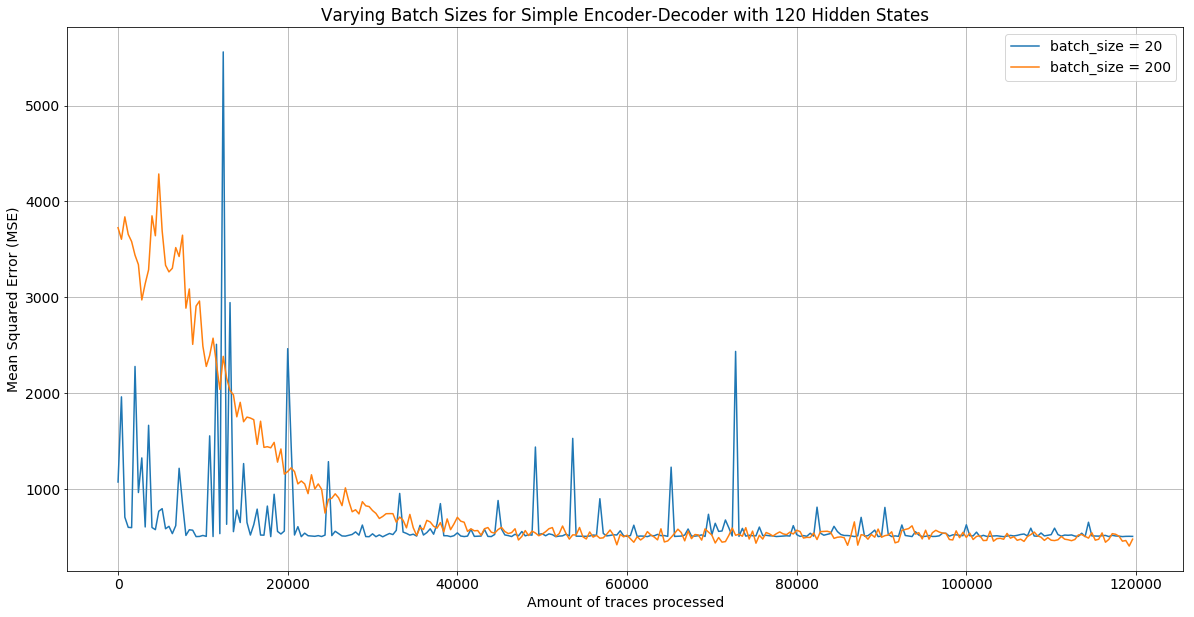
\includegraphics[width=\textwidth]{varying-batch-sizes}
  \caption{Scaled MSE over traces processed for different batch sizes.}
  \label{fig:varying-batch-sizes}
\end{figure}

Preferably we would like to have an even greater batch size than $200$ but due to memory constraints, the model runs out of memory when the amount of hidden states is greater than $100$.
Thus through the rest of the report we will use a mini-batch size of $200$.

Next, we vary the learning rate $\gamma$ from $0.01$ to $0.000001$ with various optimizers (\textit{adam}, \textit{gradient descent} or \textit{RMSProp}) and loss functions (\textit{mean squared error (MSE)} or \textit{absolute loss} (AL)).
For this, we aim to get a learning curve that gradually decreases, the more traces the model processes and eventually slows down once the model reaches a minimum.

After trying a wide variety of different permutations, an \textit{adam optimizer} continuously demonstrated better results.
We expected this since adam optimizers are computationally efficient, require a relatively little amount of memory and tend to perform very well with problems that have a large amount of parameters \cite{kingma2014adam},
which is ideal since our network can be unrolled to a very large lengths.

Next, we also note that the best quality of data compression was achieved with a \textit{MSE loss function} and a learning rate of $0.000002$.
Hence, we set $\lambda = 0.000002$, $b = 200$ and use an adam optimizer with MSE for the rest of our experiments.

\subsubsection{Reversing Traces}
% TODO: Reversing traces

\subsubsection{Cutting Traces}
% TODO: Cutting traces

\subsection{Architecture Tuning}

Now that we have made a decision on which learning parameters to use, we can start changing the architecture of the sequence-to-sequence model to see which ones yield the best results.
We do need to note that we might slightly deviate from the previously chosen learning parameters for different models due to memory constraints.
But when we do, we will clearly state that this is the case.

\subsubsection{Hidden States}

We first start by examining the amount of hidden states in the network.
These directly affects the size of the fingerprints that will be extracted.
We do not want these values to be too large since this makes the network more complex and requires more computation.
On the other hand, we do not want these values to be too small either since the state vector might be too small for the network to learn anything useful.

Moreover, we also need to consider the classifiers.
The more features we introduce, the more time and data they require to learn the classification task.
Whilst if the amount of features is too low, the classifier might not be able to learn how to effectively classify any of the web pages.
Hence, we base the amount of hidden states on the amount of features used in previous WF attacks.

\begin{table}[ht]
  \centering
  \begin{tabular}{ r r } \hline
    \multicolumn{1}{c}{\textbf{Model}} & \multicolumn{1}{c}{\textbf{Features}} \\ \hline
    SVC \cite{panchenko1} & $305$ \\
    SVC \cite{panchenko2} & $104$ \\
    RF \cite{kfingerprinting} & $150$ \\
    kNN \cite{wang_cai_johnson_nithyanand_goldberg_2014} & $3737$ \\
    \hline
  \end{tabular}
  \caption{Amount of features for existing attacks.}
  \label{table:feature-wf-attacks}
\end{table}

As can be seen in table \ref{table:feature-wf-attacks}, most attacks tend to have between $100$ and $300$ features if we do not consider Wang et al.'s attack.
Thus we vary the amount of hidden states between $60$ to $140$ in steps of $20$ to see which ones yield the most appropriate results.

For these experiments we train a sequence-to-sequence model with a unidirectional encoder, LSTM cells and without cutting or reversing the traces.
The training data consists $120,000$ monitored and unmonitored web pages, which are shuffled to avoid overfitting on any specific web page.
We only train the model for one epoch, as we seem to have enough data for the model to converge within that epoch.
Hence, every sample that the model sees in the figure below is one that it has never seen before.
So we can easily determine if the model overfits on specific data.

\begin{figure}[ht]
  \centering
  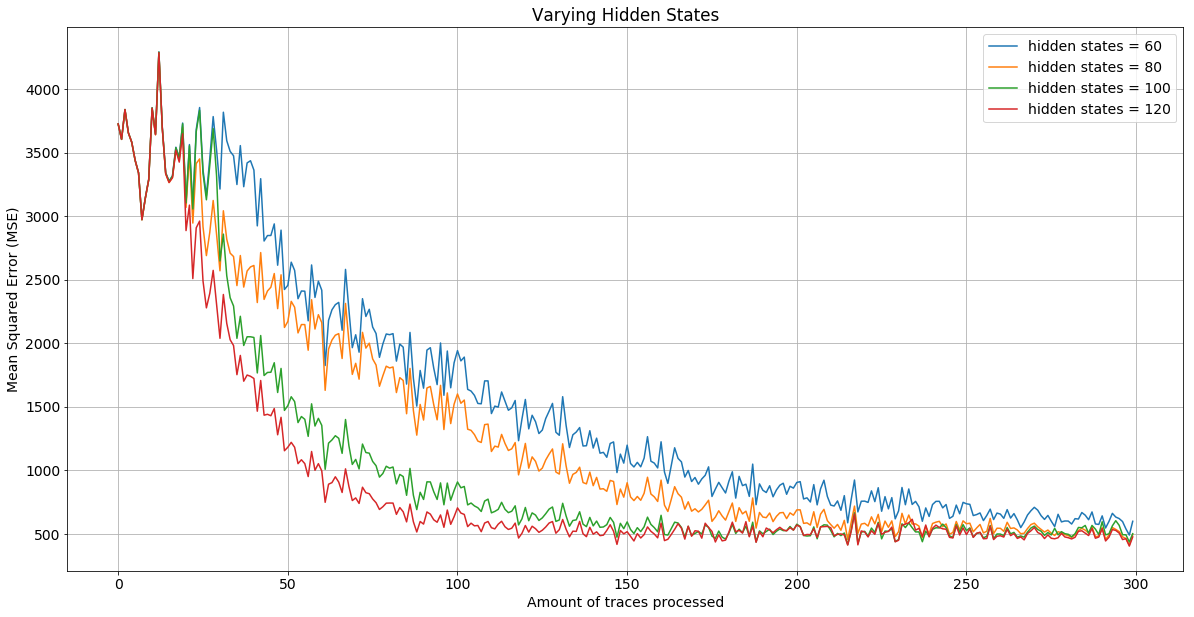
\includegraphics[width=\textwidth]{varying-hidden-states}
  \caption{MSE over the amount of traces processed for varying hidden states.}
  \label{fig:varying-hidden-states}
\end{figure}

Figure \ref{fig:varying-hidden-states} clearly shows us that the smaller the amount of hidden states, the faster the network seems to learn the reconstruction task.
This was expected because the less hidden states, the less complex the internal representation of the network is.
On the other hand, the higher the amount of states, the lower the final error seems to be.
Since we aim to compromise between computational complexity and the time it takes to train the model, around $100$ hidden states seems to be the most appropriate since it manages to a MSE that is very close to the networks with a higher amount of hidden states.

\subsubsection{Bidirectional Encoder}

Rather than using a normal encoder, a bidirectional might be more appropriate for this task.
The reasoning behind this is that for a normal encoder, the output at every cell depends on the past.
However, there might also be important information in the future that could in fact impact the output at that cell.
Thus a bidirectional encoder parses the data in both directions, which means that the output of every cell depends on both the past and the future.

The problem with this method is that it essentially introduces double the amount of free parameters as a normal encoder.
Hence, when we perform the analysis, we need to consider whether or not we should take more time waiting to train this model or whether the performance gain is not worth it.

For these experiments, we consider a smaller range of hidden state values from $80$ to $120$ in steps of $20$.
Again, for all of these we will be using LSTM cells without cutting or reversing the traces and all of the learning parameters described above and the training set will remain exactly the same.

% TODO: Add figure + conclusion

\subsubsection{LSTM or GRU Cells}

So far we've only experimented with LSTM cells since they are the most commonly used ones.
However, GRU cells have been introduced more recently.
They essentially combine several of the gates and states within LSTM cells to minimize the amount of free parameters and therefore making the model less complex.
Consequently, the model should also be able to learn fixed-length representations faster than LSTM cells.
But LSTM cells still have a greater expressive power, meaning that they could learn more complex functions.

Here, we train a sequence-to-sequence model with both a unidirectional and bidirectional encoder.
These will both have GRU cells with $100$ and $TODO: Fill in$ hidden states respectively.

Furthermore, we recreate the exact same training conditions as previously.
This means that we will not be cutting the traces nor reversing them whilst training on the same dataset of $120,000$ web pages with the previously chosen learning parameters.

% TODO: Add figure + conclusion

\subsection{Classifier Performance}

We have previously analysed the model's performance based on how well it copies the original input from a fingerprint.
But to examine how well our model performs at automatically generating fingerprints, we compare its performance on different existing classifiers with hand-picked features.
This means that we choose a set of existing WF attacks and recreate them.
Next we run the exact same attack but with the automatically generated features and various scoring statistics.

Note that our results might be slightly lower than in their respective papers since we do not aim to recreate the full attack.
Rather than optimizing different hyperparameters, we aim to use these classifiers and the hand-picked features as an indicator as to how well the sequence-to-sequence model performs.

We expect that the automatically generated features will perform worse than the hand-picked ones due to the complexity of the task.
To effectively compress a variable-length trace into a fixed-length representation is a very difficult to achieve task and due to the depth of the network, we expect that it got stuck in a local minima.
However, we still hope to show that it is in fact possible to automate this feature selection process.

As mentioned in section \ref{sec:threat-model}, there are two main threat models that we need to consider.
The first one is a binary classification task, where the adversary wants to see whether or not a user is visiting any webpages within a given set.
The other threat model involves the adversary having a set of monitored pages, and it wants to know which specific pages the user is visiting in that set.
Hence, it is a multiclass classification problem.

Although there are different techniques for evaluating binary and multiclass classification models, we will only use the scoring statistics outlined in section \ref{sec:classifier-training}.
This allows us for easy comparisons between the different threat models.
We do expect that the binary classification models will perform better than the multiclass ones due to the larger amount of options available.

Aforementioned, we have already selected a total of four different existing attacks.
We will refer to the first SVC attack by Panchenko et al. \cite{panchenko1} as \texttt{svc1} and the second one \cite{panchenko2} as \texttt{svc2}.
Whilst we refer the k-fingerprinting attack by Hayes et al. \cite{kfingerprinting} as \texttt{RF} and finally the attack by Wang et al. \cite{wang_cai_johnson_nithyanand_goldberg_2014} as \texttt{kNN}.

\subsubsection{Binary Classification}

We first start by analysing the simplest threat model, namely binary classification.
For all of the models below, we aimed to extract the exact same hand-picked features as were described in the respective papers to the best of our knowledge.

For training these models, we use an extract from the \texttt{GRESCHBACH} dataset with a total of $100$ monitored web pages with $70$ instances each and $5000$ unmonitored web pages.
We then split this set into a training and validation set using a stratified split.
The training set will contain $90\%$ of the monitored web pages whilst we vary the amount of unmonitored pages to see how the models perform.

After the set is split up into a training and validation set, we perform a \textit{stratified k-fold validation} with $k = 3$ on the training set
Then finally we train the classifiers on all of the training data and evaluate them on the test set.

The results for the k-fold validation on the training set for the hand-picked features are outlined in table \ref{table:hand-picked-bin}.
Here, we used a total of $10\%$ of the unmonitored data for training.

\begin{table}[ht]
  \centering
  \begin{tabular}{ r  r  r  r  r  r } \hline
    \multicolumn{1}{c}{\textbf{Model}} & \multicolumn{1}{c}{\textbf{Accuracy}} & \multicolumn{1}{c}{\textbf{BDR}} & \multicolumn{1}{c}{\textbf{TPR}} &
      \multicolumn{1}{c}{\textbf{FPR}} & \multicolumn{1}{c}{\textbf{F1}} \\ \hline

    \texttt{svc1} & $0.91 \pm 0.003$ & $0.99 \pm 0.001$ & $0.97 \pm 0.001$ & $0.07 \pm 0.002$ & $0.90 \pm 0.005$ \\

    \texttt{svc2} & $0.91 \pm 0.008$ & $0.99 \pm 0.001$ & $0.95 \pm 0.003$ & $0.06 \pm 0.004$ & $0.90 \pm 0.008$ \\

    \texttt{RF} & $0.93 \pm 0.003$ & $0.99 \pm 0.001$ & $0.97 \pm 0.006$ & $0.05 \pm 0.003$ & $0.92 \pm 0.005$ \\

    \texttt{kNN} & $0.90 \pm 0.007$ $0.97 \on 0.003$ & $0.94 \pm 0.004$ & $0.09 \pm 0.002$ & $0.89 \pn 0.004$ & \\

    \hline
  \end{tabular}
  \caption{Performance statistics hand-picked features on a binary classification task with k-fold validation.} % 10 % unmonitored
  \label{table:hand-picked-bin}
\end{table}

As expected, the results on the individual folds is relatively high.
However, now we will measure their performance when training on the full training set and evaluating on the validation set, whilst changing the amount of unmonitored pages we train the model on.
Since bayesian detection rate ultimately determines the feasibility of an attack, we will use that measure for comparison.


\subsubsection{Multiclass Classification}

% TODO: Finish

% TODO: Change table
\begin{table}[ht]
  \centering
  \begin{tabular}{ r  r  r  r  r  r } \hline
    \multicolumn{1}{c}{\textbf{Model}} & \multicolumn{1}{c}{\textbf{Accuracy}} & \multicolumn{1}{c}{\textbf{BDR}} & \multicolumn{1}{c}{\textbf{TPR}} &
      \multicolumn{1}{c}{\textbf{FPR}} & \multicolumn{1}{c}{\textbf{F1}} \\ \hline

    \texttt{svc1} & $0.73 \pm 0.005$ & $0.81 \pm 0.007$ & $0.81 \pm 0.010$ & $0.22 \pm 0.015$ & $0.73 \pm 0.005$ \\

    \texttt{svc2} & $0.74 \pm 0.013$ & $0.84 \pm 0.006$ & $0.76 \pm 0.016$ & $0.16 \pm 0.009$ & $0.74 \pm 0.013$ \\

    \texttt{RF} & $0.83 \pm 0.014$ & $0.93 \pm 0.014$ & $0.80 \pm 0.007$ & $0.06 \pm 0.01$ & $0.83 \pm 0.014$\\

    \texttt{kNN} & & & & & \\

    % TODO: Fill in kNN
    \hline
  \end{tabular}
  \caption{Performance statistics hand-picked features on a multiclass classification task.}
\end{table}

\subsubsection{Different Circumstances}

Beside analysing how the sequence-to-sequence model performs on data that was recorded under the same circumstances, it would be interesting to examine how it performs on other data.
It has already been shown that the performance of the classifiers is greatly impacted by the network, time and a different TBB version.
But that doesn't necessarily mean that our fingerprint extraction model is impacted similarly.

If our sequence-to-sequence model is not impacted by these flaws, an adversary would only need to train the model once and then it could continue to use it and only retrain the classifiers.
But if it were to be impacted, the retraining process would become significantly slower.

To test this premise, we use a model that we previously trained on the same $120,000$ web pages within the \texttt{GRESCHBACH} dataset.
% TODO: State architecture.
Next, we extract the fingerprints from the Tor cells within the \texttt{WANG14} dataset using this model, train a set of classifiers on these fingerprints and note down their performance.

% TODO: Include learning curve

% TODO: Classifier analysis

% TODO: Conclusion

\section{Unit Tests}

On top of evaluating the results, we also needed to ensure that the results were in fact the the code behaves as we expect it to.
For this we use unit tests.
Some of the code, such as the sequence-to-sequence model is difficult to test but we can still test all of the preprocessing to see if that is correct.
For this we use Python's standard \texttt{unittest} module \cite{python_unittest_documentation}.
The reason for this choice is that it is flexible and the standard unit testing framework, which means it is commonly used.

On top of unit tests, \textit{Travis} was also used \cite{travis}.
Travis is a popular tool, that has an easy integration with Github, for continuous integration.
Therefore, every time a commit is pushed to the remote repository, Travis runs all of the tests automatically.
If one of the tests fails, Travis then automatically notifies all the contributors.

Finally, to check if our tests cover our entire codebase, \textit{codecov} is used \cite{codecov}.
This tool automatically checks how much of the codebase all of the unit tests cover.
At the time of writing, the coverage is $93\%$.
The bits that aren't covered by unit tests, such as the Tensorflow implementation of the sequence-to-sequence model, have been carefully examined to see if they behave as expected by using the Tensorflow debugger \cite{tensorflow}.
